%! TEX root = 'main.tex'
\section{Experiment}
\label{sec:experiment}

\subsection{Reverse Engineering}
We did reverse engineering to this PLC in order to better understand it, so that it can be completely controlled. This reverse engineering consists of two parts. The hardware part is to distinguish the modules and how they are connected. The software part is mainly the disassembly of the firmware.

\subsubsection{Backplanes}

A PLC such as Allen-Bradley 1769-L18ER-BB1B/B CompactLogix 5370, usually contains multiple PCB module boards, called backplanes, as shown in~\autoref{fig:modules}.

\begin{figure}[th]
	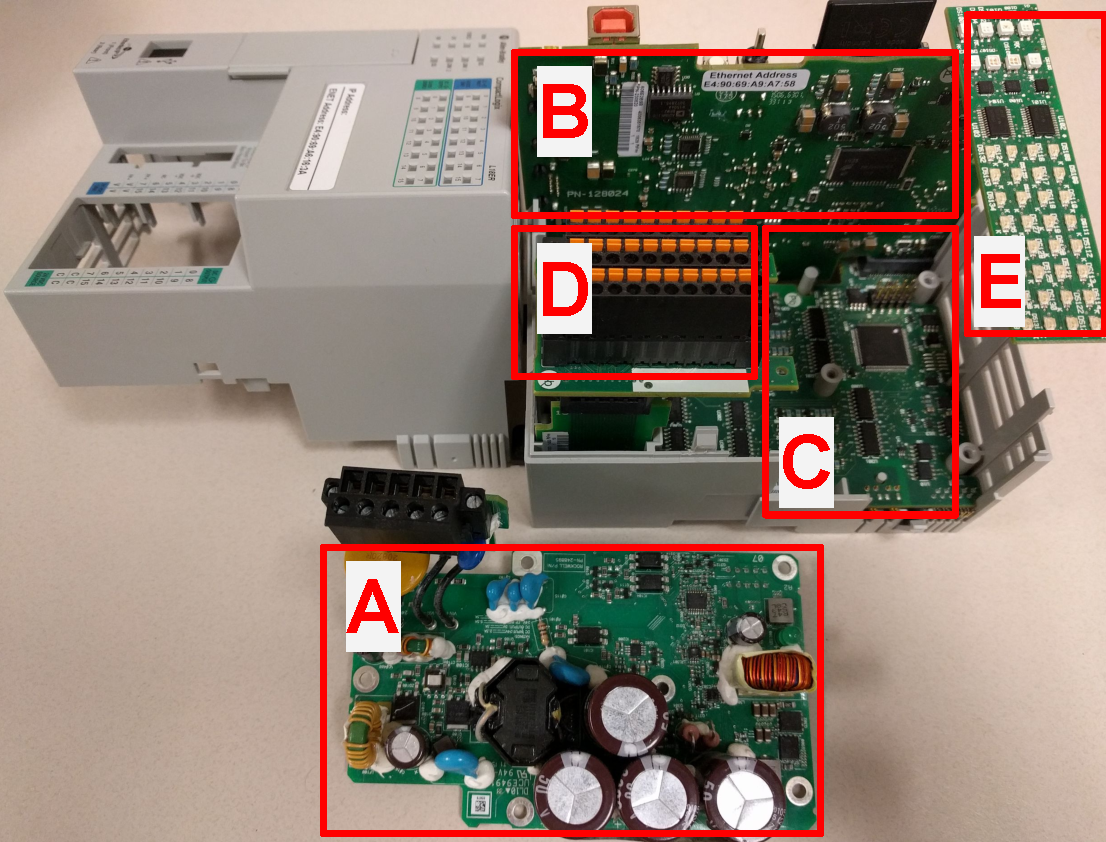
\includegraphics[width=0.47\textwidth]{figures/modules}
	\centering
	\caption{Allen-Bradley 1769-L18ER-BB1B/B CompactLogix 5370 PLC. A: Power supply module  B: Communication module  C: Real-time module  D: (16) DC Digital Outputs \& (16) DC Digital Inputs  E: LED indicator module}
	\label{fig:modules}
\end{figure}

For the PLC we use, it contains one communication module, one real-time controller module, DC digital input/output module and the power supply module. They are interconnected through a proprietary interface. The communication module itself is a complete embedded system that is responsible for communicating with external systems such as SCADA trough Ethernet. It may also host a website for statistics and management.

The real-time controller module also is a complete embedded system. It uses a real-time operating system to handle industrial logic signals though input/output module.

In this paper, because our main purpose is to control the physical system, our focus is on the real-time controller module.


\subsubsection{Microcontroller}

The real-time controller module uses the TI Stellaris LM3S2793 SoC. It has a ARM Cortex-M3 processor core operates at 80 MHz. It contains up to 67 GPIOs depending on configuration, JTAG and ARM Serial Wire Debug (SWD) interfaces, two I2C modules and so on.

\subsubsection{Internal Memory}The Stellaris LM3S2793 microcontroller~\cite{lm3s2793} comes with 64 KB of bit-banded SRAM, internal ROM, and 128 KB of Flash memory. The internal ROM is located at address 0x1000000 of the device memory map. It contains the following components:

\begin{itemize}
	\item Stellaris Boot Loader and vector table
	\item Stellaris Peripheral Driver Library (DriverLib) release for product-specific peripherals and interfaces
	\item Advanced Encryption Standard (AES) cryptography tables
	\item Cyclic Redundancy Check (CRC) error detection funtionalify
\end{itemize}

The ROM can be seen as a function library similar to the PC BIOS. Instead of calling through system interrupt, it's called by a vector table. We will talk about it in more detail later.

The LM3S2793 microcontroller provides 64 KB of single-cycle on-chip SRAM. The internal SRAM is located at offset 0x20000000 of the device memory map.

The 128 KB flash memory stores the user application code. This part is what we need to do reverse engineering. The first step is to find out where the code is and the entry point.

\begin{center}
	\begin{table}
		\begin{tabular}{|p{1.6cm} p{1.6cm} p{4cm}|} 
			\hline
			Start & End & Description \\ [0.5ex] 
			\hline\hline
			0x00000000 & 0x0001FFFF & On-chip Flash \\ 
			\hline
			0x00020000 & 0x00FFFFFF & Reserved \\
			\hline
			0x01000000 & 0x1FFFFFFF & Reserved for ROM \\
			\hline
			0x20000000 & 0x2000FFFF & Bit-banded on-chip SRAM \\
			\hline
			0x20010000 & 0x21FFFFFF & Reserved \\
			\hline
			0x22000000 & 0x221FFFFF & Bit-band alias of bit-banded on-chip SRAM starting at 0x20000000 \\
			\hline
			0x22200000 & 0x3FFFFFFF & Reserved \\
			\hline
			... & ... &   \\ [1ex] 
			\hline
		\end{tabular}
		\caption{LM3S2793 Memory Map}
		\label{tab:memorymap}
	\end{table}
\end{center}

\autoref{tab:memorymap} shows part of the memory map of LM3S2793, it's easy to see where the flash memory is. It's from 0x00000000 to 0x0001FFFF, 128 KB. But we also have to be aware that this mapping may change because of the boot loader.

The Stellaris Boot Loader is used to download code to the Flash memory of a device without the use of a debug interface. It means that when the microcontroller is rest, the user has the opportunity to direct the microcontroller to execute the ROM boot loader or the application in flash memory by using any GPIO signal in GPIO ports as configured in the Boot Configuration (BOOTCFG) register.


\subsubsection{Entry Point}
At reset, the ROM is mapped over the flash memory so that the ROM boot sequence is always executed. After that, depends on the BOOTCFG's setting and the signal from certain GPIO port, the ROM is mapped to 0x01xxxxxx and flash memory is mapped to the address 0x00000000. Then, the data at address 0x00000004 is read. If the data is 0xFFFFFFFF, which means the flash is not programmed, the ROM will be mapped back to address 0x00000000 again and execution continues out of the ROM boot loader. If it's not 0xFFFFFFFF, the data at address 0x00000000 will be used as the stack address and it will be loaded into stack pointer (SP). The program counter (PC) is loaded from address 0x00000004. That's the entry point for user application. This is also confirms to ARM's definition of vector table. ARM architecture expects the interrupt vector table at the start of the memory. It contains the reset value of the stack pointer, and the start address, also called exception vectors, for all exception handlers.  

In our device, the SP value is 0x20000B48, and the PC value is 0x000000E3. Since 0xE3 is an odd number, which violate the memory alignment of ARM architecture, the least significant bit indicates that from address 0xE2, the instruction are in Thumb code.

We dumped the flash memory to a file, and start to disassemble at address 0xE2.

We also noticed that the SRAM which starts from 0x20000000, replicate the flash memory. This is because SRAM runs much faster than the flash. At system clock speeds of 50 MHz and below, the flash memory is read in a single cycle. LM3S2793 operates at 80 MHz. But the flash memory has a prefetch buffer that is automatically used when the CPU frequency is greater than 50 MHz. In this mode, the flash memory operates at half of the system clock. The prefetch buffer fetches two 32-bit words per clock allowing instructions to be fetched with no wait states while code is executing linearly.

When the system boot, the first thing it does is to copy part of flash to SRAM, specifically, copying 0x0 - 0xA88 to 0x20000000 - 0x20000A88. Next, clears 0x20000A88 - 0x20000F54 to 0. Then it sets up the Vector Table Offset Register which contains the location of the vector table, indicating either it's in flash or SRAM and the offset. After these steps, the code jumps back to SRAM to continue execution.




\subsubsection{Stellarisware ROM Library}
The ROM library~\cite{lm3s2793rom} use tables to access function entry points for the APIs that are provided in the ROM. The tables are split into two levels. The main table contains one pointer per peripheral which points to a secondary table that contains one pointer per API that is associated with that peripheral. The main table is located at 0x01000010 right after the Cortex-M3 vector table in the ROM. \autoref{tab:romtable} shows a portion of the API table and ~\autoref{tab:gpiotable} shows part of the secondary ROM\_GPIOTABLE which contains the entry points of all the GPIO related functions.

\begin{center}
	\begin{table}
		\begin{tabular}{|p{7.2cm}|} 
			\hline
			ROM\_APITABLE (0x1000010) \\ [0.5ex] 
			\hline
			[0] = ROM\_VERSION \\
			\hline
			[1] = pointer to ROM\_UARTTABLE \\
			\hline
			[2] = pointer to ROM\_SSITABLE \\
			\hline
			[3] = pointer to ROM\_I2CTABLE \\
			\hline
			[4] = pointer to ROM\_GPIOTABLE \\
			\hline
			[5] = pointer to ROM\_ADCTABLE \\
			\hline
			... \\ 
			\hline
		\end{tabular}
		\caption{LM3S2793 ROM API Table}
		\label{tab:romtable}
	\end{table}
\end{center}

\begin{center}
	\begin{table}
		\begin{tabular}{|p{7.2cm}|} 
			\hline
			ROM\_GPIOTABLE \\ [0.5ex] 
			\hline
			[0] = function ROM\_GPIOPinWrite \\
			\hline
			[1] = function ROM\_GPIODirModeSet \\
			\hline
			[2] = function ROM\_GPIODirModeGet \\
			\hline
			[3] = function ROM\_GPIOIntTypeSet \\
			\hline
			... \\ 
			\hline
		\end{tabular}
		\caption{GPIO API Table}
		\label{tab:gpiotable}
	\end{table}
\end{center}


The following is an example of calling function ROM\_GPIOPinRead() from the flash memory disassembly. API table indexing 0x1000010 + 0x10 (ROM\_APITABLE[4]) is optimized to 0x1000020 which points to the GPIO API table. [R2,\#0x2C] represents ROM\_GPIOTABLE[11] which is ROM\_GPIOPinRead(). So the code that calling the ROM library is very helpful to reveal the intent of the program.


\begin{figure}[th]
	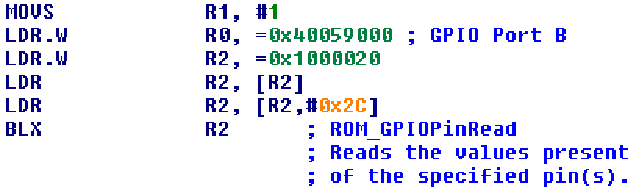
\includegraphics[width=0.47\textwidth]{figures/romapiexample}
	\centering
	\caption{Example of calling ROM library API}
	\label{fig:romapiexample}
\end{figure}



\subsubsection{Debugging}

Debugging plays an important role in the reverse engineering process. To debug an ARM core, we need the JTAG interface and a hardware debugger. In this project, we use SEGGER J-Link which contains a GDB-Server. The J-Link GDB Server is a remote server for the GDB which allows to use J-Link with GDB or any tool chain which uses GDB as debugging interface. We also need GNU Embedded Toolchain for ARM~\cite{gnutoolchainarm}, meaning, the ARM version of gdb client.

As mentioned earlier, the stack pointer and program counter are located at address 0x00000000 and 0x00000004 which is the reset vector. To debug the target ARM core, we use a GDB initialization script, as shown below, which contains GDB commands to automatically execute during GDB startup to make the debugger stopping at the beginning of the reset vector.  

\begin{lstlisting}[basicstyle=\small, caption={GDB stript file .gdbinit}, captionpos=b]
target remote localhost:2331
monitor speed 1000
monitor reset
monitor reg r13 = (0x00000000)
monitor reg pc = (0x00000004)
monitor flash breakpoints = 1
\end{lstlisting}

At this point, if you enter the gdb command "continue", the ARM core will continue to execute and then run ladder logic normally. But whenever you interrupt the core with hitting "Ctrl - C", the red LED of the PLC will light up and report an IO error. 


\subsubsection{more reverse engineering topics ....}

Through reverse engineering, it shows that the Vector Table Offset Register is first at address 0x0, then switch to address 0x20000000, after receiving the ladder logic code, finally set to address 0x40000. 

\subsection{GPIO}
The most important way for PLC to control the physical system is through the input and output pins on the IO module. These pins correspond directly to the GPIO on the real-time microcontroller. So, knowing how to control GPIO and having knowledge of the physical system is equivalent to being able to directly control the physical system.

The way to control GPIO is different on different microcontroller. Luckily it's well documented for LM3S2793 microcontroller~\cite{lm3s2793}. 

There are up to 67 GPIOs, depending on configuration. They can be used individually as GPIO pins or one of several peripheral functions by pin muxing.

There are multiple registers associated with each GPIO port. For instance, GPIO port mode register, GPIO port data register, GPIO bit set/reset register and so on. Those registers are used to configure and hold the data for the GPIO port. Usually when we configure the registers, we use the "Read Modify Write" (RMW) where we need to first read the register, and then, depending on the value, a new value will be write back to the same register. But most of the microcontroller doesn't have an atomic RMW operation. If multiple pieces of code are running at the same time, especially on multiprocessor systems, it will cause synchronization problems (Race condition). To address the issue, some GPIO module has Bit Set/Reset Register (BSRR) or Bit Reset Register (BRR). For example, the BSRR could be a 32-bit register where the lower 16 bits are used to set any of the 16 pins of a particular GPIO port, and the higher 16 bits are used to clear the same 16 pins.

The LM3S2793 uses a different approach. The GPIO ports allow for the modification of individual bits in the GPIO Data (GPIODATA) register by using bits [9:2] of the address bus as a mask. In this manner, software drivers can modify individual GPIO pins in a single instruction without affecting the state of the other pins. This explains why a GPIO port requires a large address space, because to implement this method, the GPIODATA register covers 256 locations. 

During a write, if the address bit associated with that data bit is set, the value of the GPIODATA register is altered. If the address bit is cleared, the data bit is left unchanged. For example, writing a value of 0xEB to the address GPIODATA + 0x098 has the result shown in~\autoref{fig:gpiowrite}, where u indicates that data is unchanged by the write. 

\begin{figure}[th]
	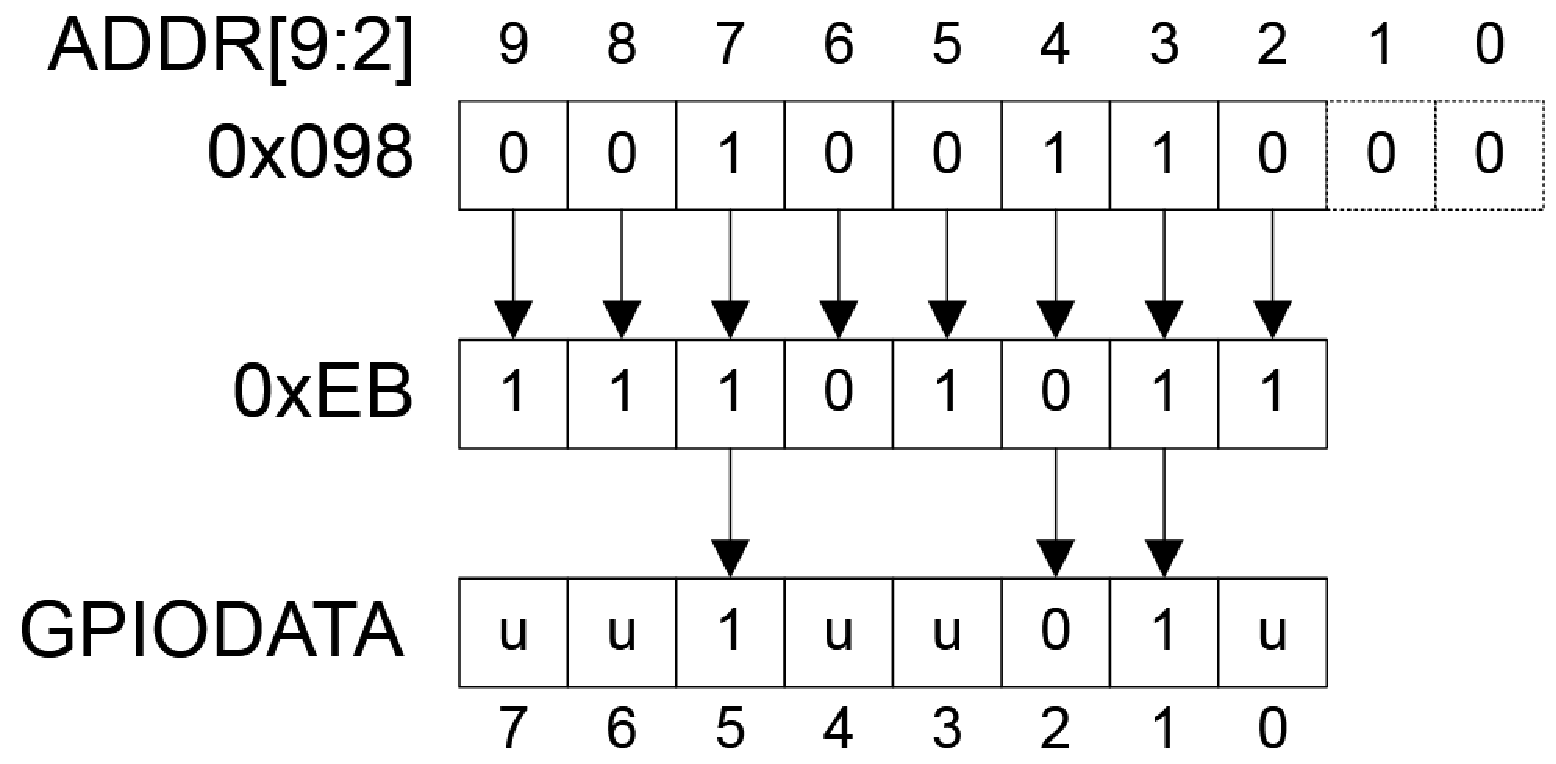
\includegraphics[width=0.47\textwidth]{figures/gpiowrite}
	\centering
	\caption{GPIODATA Write Example~\cite{lm3s2793}}
	\label{fig:gpiowrite}
\end{figure}

During a read, if the address bit associated with the data bit is set, the value is read. If the address bit associated with data bit is cleared, the data bit is read as a zero, regardless of its actual value. For example, the result for reading address GPIODATA + 0x0C4 is shown in~\autoref{fig:gpioread}.

\begin{figure}[th]
	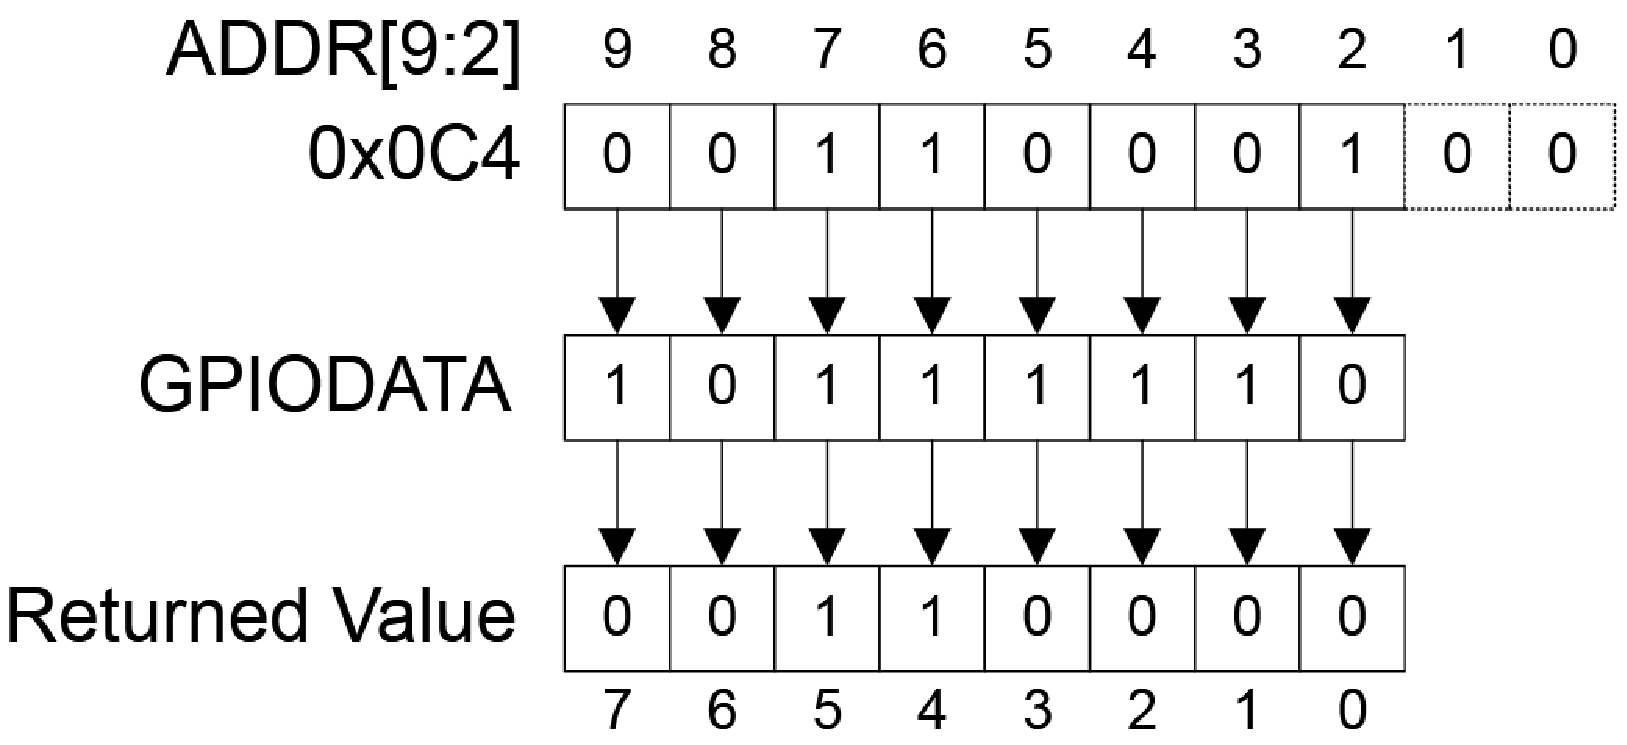
\includegraphics[width=0.47\textwidth]{figures/gpioread}
	\centering
	\caption{GPIODATA Read Example~\cite{lm3s2793}}
	\label{fig:gpioread}
\end{figure}



\subsection{Attacks}
After controlling JTAG, there are many ways to attack. One of the attacks is to change the IO output without changing the panel LED indicator and monitoring system. Through reverse engineering, we know that GPIO port E (0x4005C000), GPIO port F (0x4005D000) corresponds to IO inputs, and GPIO port G (0x4005E000), GPIO port H (0x4005F000) corresponds to IO outputs. Each GPIO port contains 8 effective bits, corresponding to each pin on the panel. As mentioned earlier, we can change the GPIO output by changing the GPIO Data (GPIODATA) register. For instance, to modify all the pins on GPIO port G, write a byte to address 0x4005E3FC. For each bit in the byte, zero means output field power voltage, 1 means output low voltage (8v).

The scan cycle is the cycle of which the PLC gathers the inputs, runs the ladder logic and then updates the outputs. Scan cycles repeat in milliseconds. It will update the outputs based on the ladder logic, here ladder logic refers to variables in memory. With some reverse engineering work, we can modify those variables accordingly to get the IO output we want. We also found an particular variable that controls the update of IO output. For example, this variable in our case is located at 0x20002D0B, it varies due to different firmware version. When this variable is set to 0, the IO module stops at the current state. So now we can change the output arbitrarily. After changing this variable back to the original value, everything is restored to the state corresponding to the ladder logic. So we have a time window of arbitrary length for malicious output. 



\subsection{Onboard Components Interconnection}
Knowing how the real-time controller controls IO module, how to attack attack through the JTAG interface, we hope to learn more about the other chips on the board and how the different backplanes are related. We found that no other chips are daisy chained together with LM3S2793 via JTAG, so we need more reverse engineering work.

\subsubsection{AT45DB021E SPI Serial Flash Memory}
Right next to the LM3S2793 microcontroller, there is a flash chip, "adesto 45DB021E SHN" printed on it. It's a 2-Mbit SPI serial flash memory chip. According to the pin diagram of the LM3S2793 and AT45DB021E and the multimeter connectivity test, we found that the flash chip is connected to the SSI0 (Synchronous Serial Interface) of LM3S2793 as shown in~\autoref{fig:ssi0}.

\begin{figure}[th]
	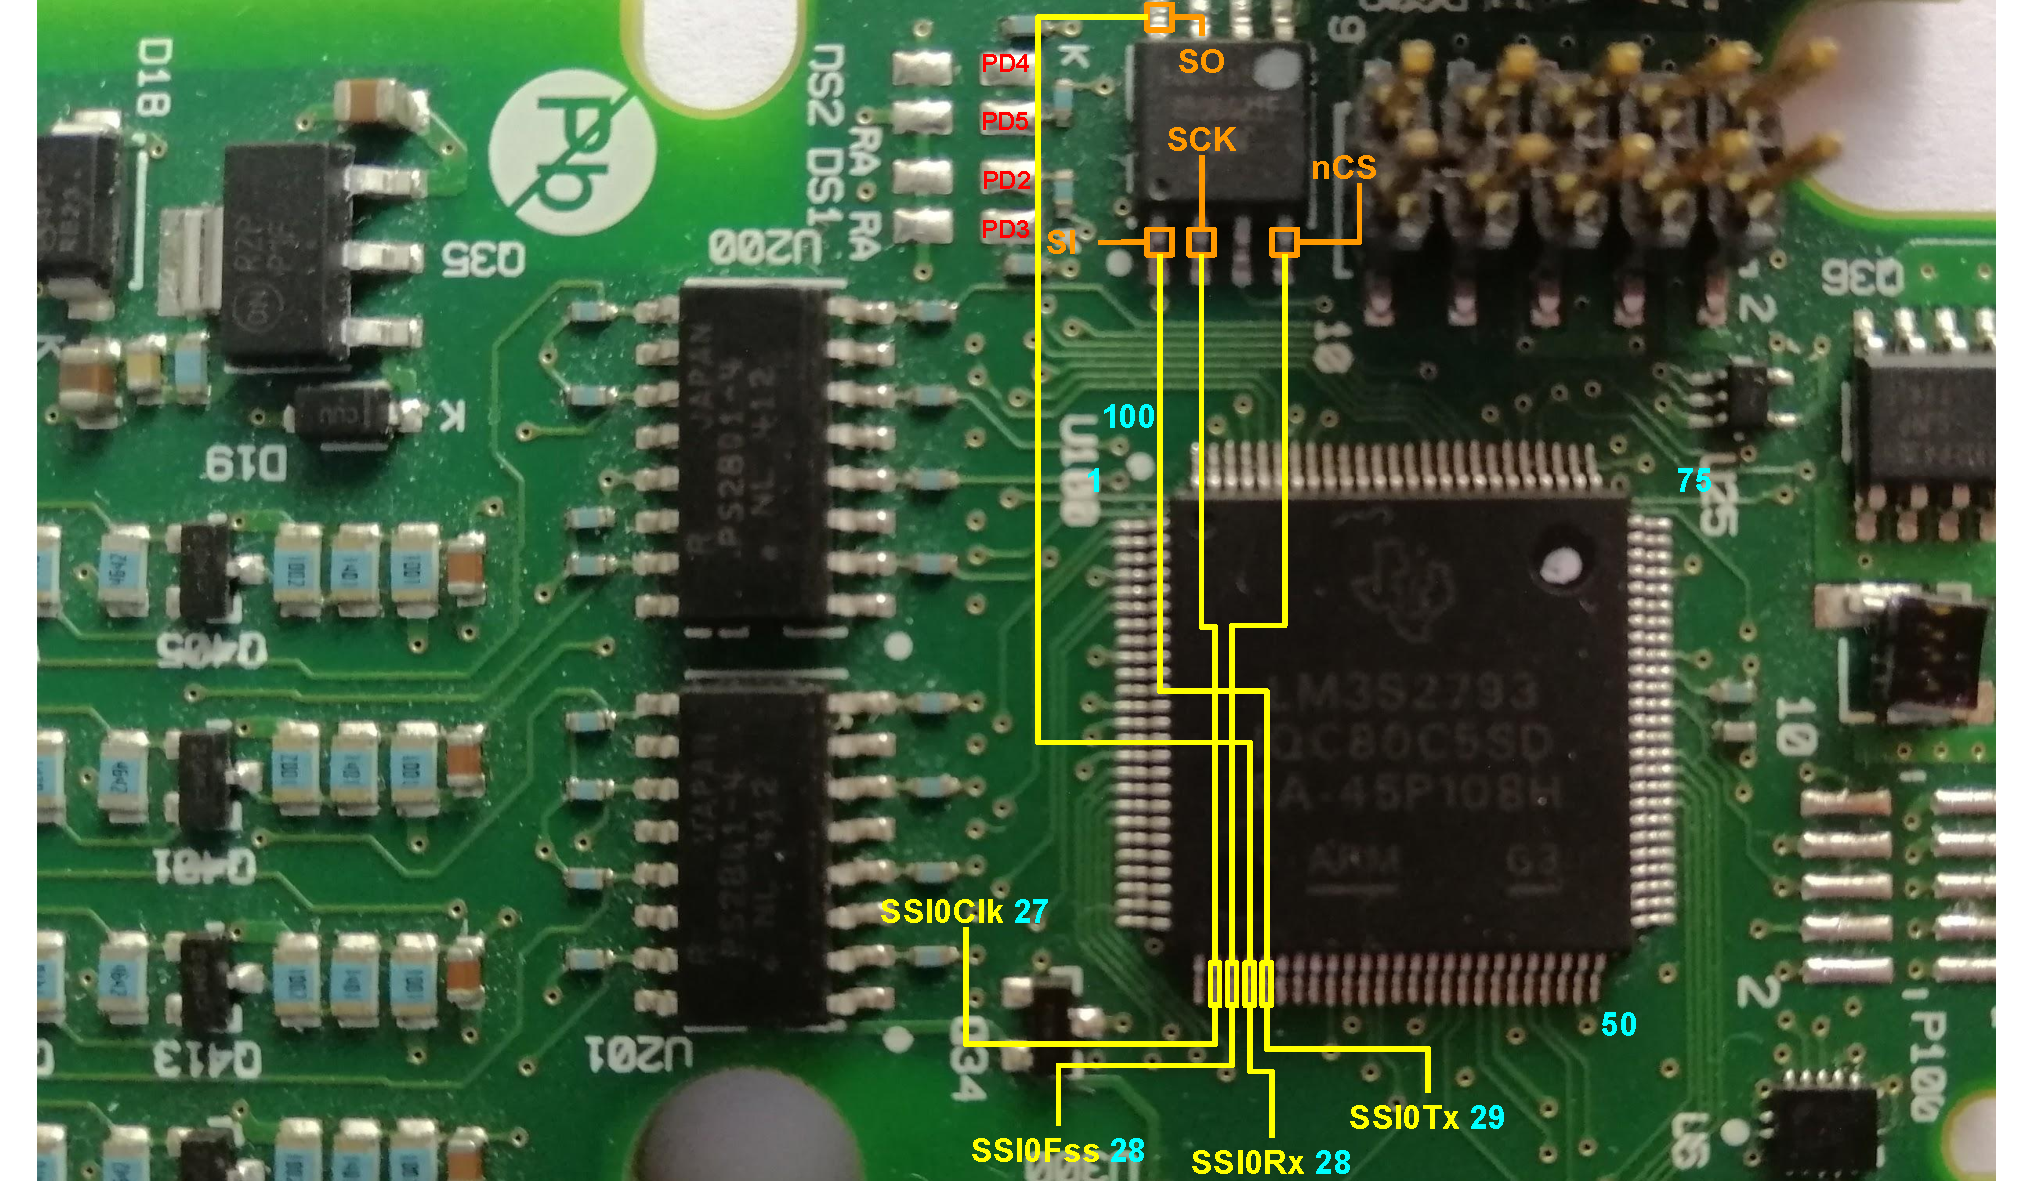
\includegraphics[width=0.47\textwidth]{figures/ssi0}
	\centering
	\caption{LM3S2793 SSI0 Pins Connect to AT45DB21E SPI Serial Flash Memory}
	\label{fig:ssi0}
\end{figure}

Also, at the beginning of the firmware initialization, right after copy part of the inner flash to RAM as we mentioned earlier, by associating GPIO port A and SSI0, the firmware first read a byte from the flash chip (from the first byte of page 128). This byte is stored at address 0x20000F50. If the value of this byte is 0x55 or 0xAA, the firmware will skip the checksum of 0x4000 to 0x1FFFC. 

The checksum is very simple. From 0x4000 to 0x1FFFC, accumulate each byte, and the final result is compared with the byte at 0x1FFFF. If they are equal, the check passes.
